\documentclass{article}
\usepackage{listings}
\usepackage{graphicx}

\newcommand{\SolutionName}{Rational}
\newcommand{\ProjectName}{Rational}

\newcommand{\code}[1]{\lstinline{#1}}

\title{\ProjectName{} Runtime Checking Example}
\date{}


\begin{document}
\maketitle
\begin{abstract}
This example shows how to enable different levels of runtime checking
in your projects.
\end{abstract}

\newcommand\codefamily\sffamily
\lstset{language={[Sharp]C},mathescape=true,flexiblecolumns=true,morekeywords={Requires,Ensures,Invariant},basicstyle=\codefamily\small,literate={->}{{$\rightarrow$}}{2}{<<}{{$\langle$}}{2}{>>}{{$\rangle$}}{2}{!}{{\textbf{!}}}{2},frame=lines,moredelim=[is][\itshape]{@}{@},captionpos=b,numberstyle=\tiny,stepnumber=1,numbersep=2pt}

\section{Adding the Contract Library Reference}
If you are using Visual Studio 2008, or if you for 
some reason want to target a pre-v4 .NET runtime, then you need to:
\begin{itemize}
\item Change the target framework of the project.
\item Manually add a reference to Microsoft.Contracts.dll
\end{itemize}
Otherwise, you may skip this section and go directly the next section!

To add the reference, open the
\textsf{\SolutionName{}} solution and right-click on
\textsf{References} in the \textsf{\ProjectName{}} project and
select \textsf{Add Reference}. Find the \textsf{Microsoft.Contracts}
library in the \textsf{.NET} tab as shown below and click OK.
\begin{center}
  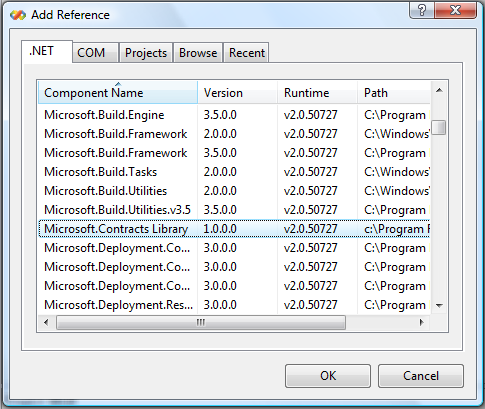
\includegraphics[width=.7\columnwidth]{../Common/addRef.png}
\end{center}



\section{Sample Walkthrough}
\label{sec:start}

\subsection{Full Contract Checking}
After adding the proper reference, go to the Properties of project
\textsf{\ProjectName}, select the Code Contracts pane (at the bottom),
and enable runtime checking. Set the runtime checking level to
\textsf{Full}. This will check all contracts at runtime, including
precondititions, postconditions, invariants, asserts, and assumes.
\begin{center}
  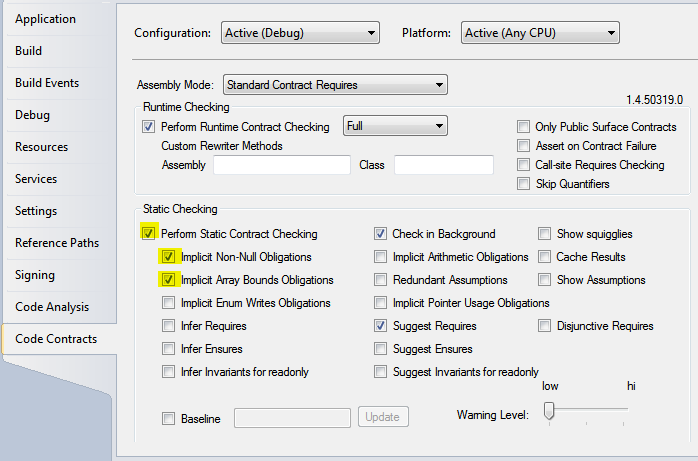
\includegraphics[width=.8\columnwidth]{ex1.png}
\end{center}
Build and run the solution (e.g. by simply hitting F5). You should get
the following dialog:
\begin{center}
  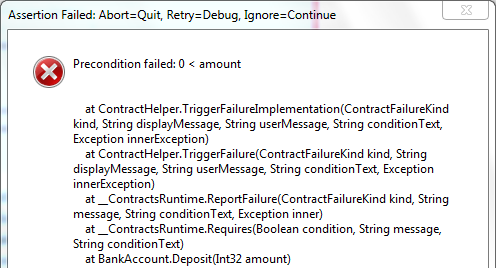
\includegraphics[width=.8\columnwidth]{ex2.png}
\end{center}
stating that some invariant is violated. To debug this case, click
\textsf{Retry} and look at the call stack. We are in the
\code{PositiveDenominatorInvariant} method, which states that
\code{PositiveDenominatorRational} expects to always have a positive
denominator. Obviously, we somehow failed to maintain this invariant.

If you look at the call frame below, you notice that we are in the
\code{Divide} method after the call to \code{base.Divide}. Since the
\code{divisor} argument is negative (-5) and the base class simply
multiplies the denominator with that value, we ended up with a
negative denominator. So the \code{Divide} override must reestablish
the invariant before returning.

We could fix the code at this point, but that is not the purpose of
the sample. So let's stop the debugging session for now, but observe
that the bottom of the call stack is located in the \code{Main} method
at line 18.

\paragraph{What happened under the hood?} The build instructed the compile
of the project to include contracts. A post-build step
then rewrote the project assembly to perform the checks in the proper
positions (e.g., invariants on exit of public methods, post-conditions
at method exits), as well as
inheritance of all the contracts. Additionally, the rewrite step also
introduces strings of the contract conditions so that they are
available at runtime when a failure occurs.

\subsection{Checking Only Preconditions}
Go back to the \textsf{Code Contracts} property pane of the project
and change the checking level to \textsf{Preconditions} by using the
drop-down menu.
\begin{center}
  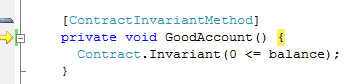
\includegraphics[width=.7\columnwidth]{ex3.png}
\end{center}
Now let's run the example again (hit F5). This time, we get a
different failure:
\begin{center}
  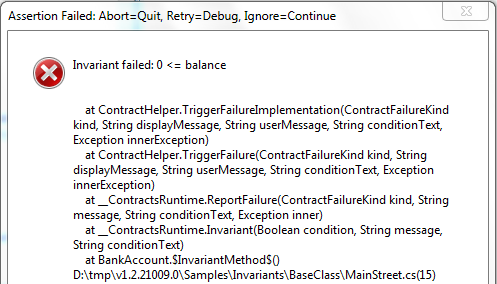
\includegraphics[width=.7\columnwidth]{ex4.png}
\end{center}
click \textsf{Retry} to enter the debugger and see where we are
failing a precondition. We notice that we are in the constructor of
\code{PositiveDenominatorRational} and parameter \code{d} is
0. Looking at the call stack below, we see that we are now at line 20
in the \code{Main} method. Thus, by checking only preconditions, we
skipped over the invariant check that failed when checking
\textsf{Full} contracts.

\paragraph{What happened under the hood?} The build instructed the compile
of the project to include contract calls. The assembly was
then rewritten to retain only precondition checks (including inherited
ones) and remove all other
contract checks. Additionally, the proper condition strings were inserted so that they are available
at runtime.

\pagebreak[1]
\subsection{Checking Only ReleaseRequires}
Stop the debugging session and go back to the \textsf{Code Contracts}
property pane and select \textsf{ReleaseRequires} as the checking level
in the drop-down menu. This level includes only preconditions of the
form \code{Requires<E>} and legacy-preconditions of the form
\code{if-then-throw}\footnote{Due to the older contract class in
  VS2010 Beta1, we also temporarily include \code{RequiresAlways}}.

Rebuild and run by hitting F5 again. This time, we hit yet another
problem.
\begin{center}
  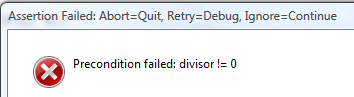
\includegraphics[width=.7\columnwidth]{ex5.png}
\end{center}
Click \textsf{Retry} to enter the debugger and notice that we are now
in the \code{Divide} method of the \code{NormalizedRational}
class (look at the call stack). The source line the debugger is
stopped on however is the base class \code{Divide} method, which specifies
the precondition \code{divisor != 0}. There are several things to note
here:
\begin{itemize}
\item The precondition \code{divisor != 0} was inherited from the base
  method \code{Rational.Divide} into the overriding method
  \code{NormalizedRational.Divide}

\item The precondition was specified as an \code{if-then-throw}. Due
  to the presence of the call \code{Contract.EndContractBlock}, this
  ``legacy-requires'' was recognized by the tools as a proper
  precondition.

\item Because the default behavior for contract failure in this build
  is set to \emph{assert} (checkbox on Contract Property Pane), even
  this legacy-requires (if-then-throw) produces an assertion. This is
  useful to detect contract failures in tests that would otherwise be
  hidden by catch handlers.

\end{itemize}


\paragraph{What happened under the hood?} The build instructed the compile
of the project to include contract calls.
The assembly was then rewritten to retain only \code{Requires<E>}, and
legacy-requires, while removing all other contract checks. The rewrite
also performed contract inheritance of these preconditions
and inserted the proper condition strings so that they are available
at runtime. Because the selected runtime failure behavior of contracts
was set to \emph{assert}, the instrumented failure behavior was to
call \code{System.Debug.Assert} instead of throwing exceptions. 

\subsection{Setting Contract Failure to Throw}
Quit the debugger and go back to the \textsf{Code Contracts} property
pane again. This time, change the runtime contract failure behavior to
throw exceptions by clearing the box ``Assert on Contract Failure'':
\begin{center}
  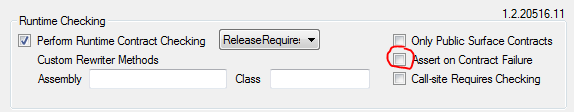
\includegraphics[width=.8\columnwidth]{ex6.png}
\end{center}
Rebuild and run the project by hitting F5 again. This time, you should
see a failure of the following form:
\begin{center}
  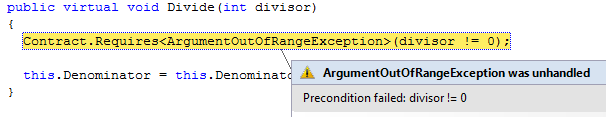
\includegraphics[width=.8\columnwidth]{ex7.png}
\end{center}
The expected exception is thrown to indicate the contract
failure. Because this is a legacy-requires, the failing condition
string is not included in the exception message. 
Other contract failures do throw \code{ContractException} and include
the failing condition string at runtime.

\section{Setting Checking Level to None}
Setting the runtime checking level to \emph{None} in the contract pane
builds a version of your code where all contract checks are removed,
\emph{including} legacy-requires. 
\begin{center}
  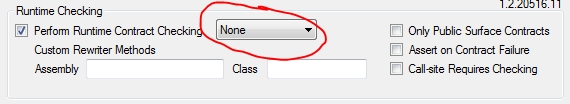
\includegraphics[width=.8\columnwidth]{ex8.png}
\end{center}
Try it out by setting the level to
\emph{None} and hitting F5. In this build and run, there were not
enough argument validations, and we fail a division by zero somewhere
deep in the code.
\begin{center}
  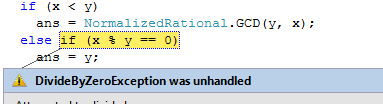
\includegraphics[width=.8\columnwidth]{ex9.png}
\end{center}
Runtime checking level \emph{None} is therefore not recommended for
anything but determining performance of your application without any
contracts enabled.

\section{Disabling Contract Runtime Checking}

Quit the debugger and go back to the \textsf{Code Contracts} property
pane again. This time, turn off the runtime contract checking completely:
\begin{center}
  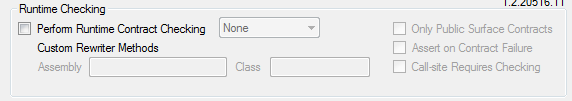
\includegraphics[width=.8\columnwidth]{ex10.png}
\end{center}
Rebuild and run the project by hitting F5 again. This time, you should
now see the legacy-requires failing as earlier.
\begin{center}
  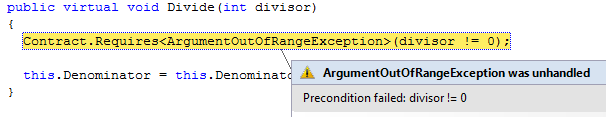
\includegraphics[width=.8\columnwidth]{ex7.png}
\end{center}
A small difference  with respect to the earlier version where we
enabled runtime checking with level \emph{ReleaseRequires} is that in
this build without runtime contract checking turned on, no contract
inheritance is performed. Thus, the check fails slightly later, namely
when \code{NormalizedRational.Divide} calls \code{base.Divide}. If the
overriding method were not calling the base method at all, the check
would be lost in this build.

For release builds where runtime contract checking is disabled, the
programmer is responsible for inheriting the argument validations (as
in current practice). See Section 5 of the Code Contracts User Manual
for more information about how to use Code Contracts effectively in
your project.

\paragraph{What happened under the hood?} With runtime checking
disabled, the build instructed the compile 
of the project to include no contract calls whatsoever. As a result,
only legacy-requires are included in this build.

\subsection{Summary}
Different levels of runtime checking are available to accomodate
particular testing or shipping needs. The more checking that is
enabled, the earlier failures are detected.
\end{document}
